\chapter{Search for semi-visible jets}  % might want to be more specific with the title if it only considers the generator-level studies
\label{chap:svj}

\epigraph{Of darkness visible so much be lent, as half to show, half veil, the deep intent.}{--- Alexander Pope}

\initial{T}his is the analysis chapter on \glspl{svj}.

%=======
\begin{easylist}[itemize]
    \easylistprops
    & Not 100\% sure whether this should go between theory and detector chapters, between detector and objects, or between objects and Hinv.
    && This could even be appended onto to the SVJ bit in the theory chapter, instead. Though, there would be a reasonable amount of material and discussion, so probably deserves its own (short) chapter
    & Only really discuss my contributions: $s$- and \tchannel signal model production and understanding. Can go into reasonable detail -- at the level of the AN or perhaps deeper
    && Show \schannel comparisons between \MADGRAPH and \PYTHIA, as shown in the AN, and discuss merits of using either method (easier to specify in \PYTHIA and matrix element calculations should be equivalent to \MADGRAPH, but latter is required for \tchannel and makes sense to have consistency)
    && Show a few distributions from \tchannel signal, just for some insight as to how they differ from \schannel. Not sure if they need some sort of approval since they're generated with \acrshort{cmssw}
    && Note that these are before any cuts, so comparing right what comes out of the generator + \acrshort{cmssw} processing pipeline. Could even potentially make some plots after applying analysis preselection that could clean up some events
    && Objects (AK4 jets, AK8 jets, MET) are straight out of nanoAOD, without the further processing and quality cuts that go into the Hinv objects. Though, since the objects have gone through the full CMSSW processing pipeline, there should be at least some intrinsic level of quality of the objects.
    && Note that we use SVJ\_3000\_20\_0.3\_peak in the analysis as benchmark point (see AN for \emph{why}). Theorists use 1000\_10 (rinv ?, alpha\_d ?). Tending to vary points around that. Note the convention for labelling the mass points: SVJ\_$\expval{m_{\mathrm{mediator}}}$\_$\expval{\mDark}$\_$\expval{\rinv}$\_$\expval{\aDark}$.
    && Also say that my \MADGRAPH implementation has been built upon for the upcoming \tchannel and boosted \PZprime searches
    & Perhaps give a brief summary of the analysis: dijet search, using an SVJ tagger, transverse mass as fit variable. Say that details/complete description is discussed in the paper/Giorgia's thesis (with references)
\end{easylist}

% Can pull from Section 35 of my lab book, and all the talks I and other people from the team have given (Presentations and talks/ folder, also Other peoples/ subdirectory). Can also pull from AN for theory, translation of some theory stuff into experiment, and analysis strategy


%=========================================================


\section{Analysis summary}
\label{sec:svj_overview}


%=========================================================


\section{Signal simulation}
\label{sec:signal_sim}

In the main analysis for the \schannel signal model, \PYTHIA is used as it can parametrise all the relevant aspects of the model in a simple manner with high efficiency. \MADGRAPH is the often-preferred generator as it can handle more complex models and decays. For the \schannel mode, the scattering matrix element calculations that model the hard process are identical between \PYTHIA and \MADGRAPH. In the former, the characterisation, interactions, and decays of the dark sector particles are implemented via the \texttt{Hidden Valley} module, available from \PYTHIA~8.226. Samples generated with \MADGRAPH are hadronised by \PYTHIA as part of the full simulation chain within \acrshort{cmssw}. \Gls{jet} matching and filter efficiencies may noticeably reduce the final number of events . The \tchannel model is possible to parametrise in \PYTHIA, but due to its complexity, we opt to do so in \MADGRAPH. Hadronisation, however, is still performed by \PYTHIA. % large number of subprocesses and potential diagrams in t-channel

The full description of \schannel signal generation with \PYTHIAEIGHT is given in Chpt.~\ref{subsec:svj_signal_pythia}. An equivalent implementation where the hard scatter is modelled in \MGvATNLO, as both an alternative and cross-check to the \PYTHIA [version], is [described] in Chpt.~\ref{subsec:svj_signal_madgraph}. A description of the \tchannel process is also present. Comparisons between the \PYTHIA and \MADGRAPH implementations are [given] in Chpt.~\ref{subsec:svj_schannel_comparisons}.

% Mention these signals are generated privately?


%=========================================================


\subsection{Generation in \texorpdfstring{\MADGRAPH}{MadGraph}}
\label{subsec:svj_signal_madgraph}

% Generating s-channel samples from my repo should be pretty consistent with Kevin's

% Mention xqcut as it relates to the qCut in Pythia. See https://answers.launchpad.net/mg5amcnlo/+question/264266

% Mention that only the hard scatter of qq -> Z' -> chi chi + (nothing, j, jj) is done in MadGraph. All hadronisation is done in Pythia. Check MadGraph run cards and FeynRules files for any interesting info

% Able to generate s- and t-channel signal in MadGraph and Pythia for 2016, 17 and 18. Important since it's a full Run-2 analysis

% Add t-channel plots as well, potentially with s-channel overlaid to show how different signals are


%=========================================================


\subsubsection{\texorpdfstring{\schannel}{s-channel}}
\label{subsubsec:svj_signal_madgraph_schannel}

% Might not be any point showing only s-channel MadGraph signal since the curves are given in the comparison plots. Though, I could instead showcase some plots from the benchmark mass point, and variations around that (e.g., vary mZp up and down by a factor of 2, then same with m_dq, r_inv, and then alpha_d_low and alpha_d_high)


%=========================================================


\subsubsection{\texorpdfstring{\tchannel}{t-channel}}
\label{subsubsec:svj_signal_madgraph_tchannel}

% Will have to decide whether to show s-channel and t-channel on same axes, or separately


%=========================================================


\subsection{Generation in \texorpdfstring{\PYTHIA}{Pythia}}
\label{subsec:svj_signal_pythia}

The \texttt{Hidden Valley} module allows for simulating $\HepProcess{\Pquark\APquark \to \PZprime \to \Pqdark\Paqdark}$, where the $\PZprime$ is acts as intended---a portal between the visible and dark sectors. Since we expect a small percentage of them to decay visibly, a branching ratio to each of the six \acrshort{sm} quarks is set to 0.003. The remaining fraction of 0.982 decays to $\Pqdark\Paqdark$, where $\Pqdark$ is a Hidden Valley particle charged only under that gauge group. The masses of the \PZprime and \Pqdark, and the narrow width of the \PZprime for resonance can be given. Showering in the dark and visible sectors is then performed as in Chpt.~\ref{subsec:svj_showering_pythia}.


%=========================================================


\subsection{Showering in \texorpdfstring{\PYTHIA}{Pythia}}
\label{subsec:svj_showering_pythia}

% Applies to both MadGraph- and Pythia-generated samples

Once the hard process has been simulated, hadronisation of the dark and visible particles is performed. Dark quarks hadronise into one of two types of dark meson that correspond to particles from the \texttt{Hidden Valley} module: \Ppidark and \Prhodark, that are pseudoscalar and vector, respectively. Each possess flavour-diagonal and off-diagonal variants. They are generated with a ratio of 1:3 as the theory specifies the number of dark flavours $\Nf = \text{2}$. Dark hadrons are set to decay invisibly with a branching fraction \rinv. Remaining decay modes are to \acrshort{sm} quarks via a virtual \PZprime since it is the leptophobic portal between the dark and visible sectors. Decays of \Prhodark are democratic, i.e., with equal probability to accessible \acrshort{sm} quark-antiquark pairs.\footnote{Top quarks are excluded in all cases, since in the scan of model parameters where we predict the greatest sensitivity, the dark mesons are always too light to decay on shell to a \ttbar pair.} Specifically, \Prhodark particles with $\mDark > \text{2}m_{\Pbottom}$ have a $\text{1}/\text{5}$ probability to decay to a \Pup, \Pdown, \Pcharm, \Pstrange, or \Pbottom. For $2m_{\Pcharm} < \mDark < 2m_{\Pbottom}$, \Pbottom quarks are excluded and the branching ratio increases to $\text{1}/\text{4}$ for the remaining species. The \Pcharm quark is removed, and branching ratio modified, in the same manner for $\mDark < 2m_{\Pcharm}$.

The decays of the \Ppidark mesons, however, are through a mass insertion. They couple to the longitudinal component of the \PZprime, assumed to arise from a leptophobic Higgs sector in an analogous manner to the electroweak bosons. Running quark masses are accounted for---as calculated in Ref.~\citenum{QCD_ESW}--since the decays are produced at the Higgs mass scale. Branching fractions to the \acrshort{sm} quarks are therefore based on the squares of the \emph{running} masses over the \emph{pole} masses. A graphical representation of the mass insertion decay is provided in Fig.~\ref{fig:svj_mass_insertion}.

% The mass insertion is briefly mentioned in the theory paper. Vector dark hadrons can decay promptly to SM quarks through the vector portal via the Z'. But scalar and pseudoscalar decays are suppressed by the mass insertion. Not sure how this affects the t-channel

\begin{figure}[htbp]
    \centering
    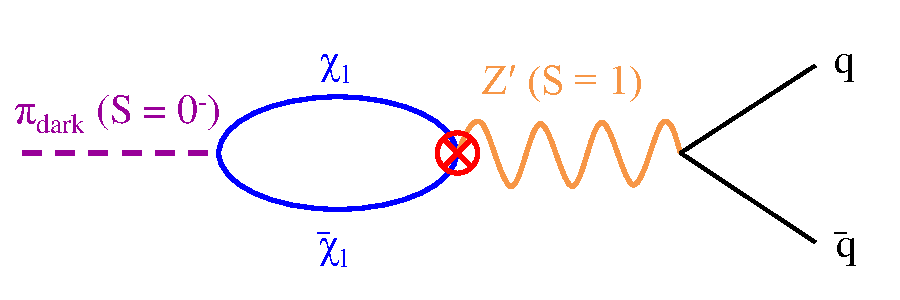
\includegraphics[width=0.5\textwidth]{figures/mass_insertion_diagram.pdf}
    \caption[A diagram of the mass insertion decay of \Ppidark mesons in the \schannel semi-visible jet model]{A diagram of the mass insertion decay of \Ppidark mesons in the \schannel \gls{svj} model.}
    \label{fig:svj_mass_insertion}
\end{figure}

We encode the dark confinement scale \lamDark and running dark coupling \aDark, based on the dark quark mass. \PYTHIA is now aware of the energy scales by which to hadronise and decay the dark sector particles. Final state dark radiation is also allowed, with a minimum \pt of $\text{1.1}\lamDark$.

% Why do we choose 1.1*Lambda_d for pt_min FSR?

The softer, visible radiation is simulated, and the clustering of \acrshort{sm} hadrons into \glspl{jet} happens. The procedure for clustering is known as ``sequential recombination'', where particles are successively combined until certain criteria are met. In \PYTHIA, clustering stops above the merging scale, which we set to 125\GeV. Referring to the transverse momentum, the symbol $\kt$ is traditionally used in naming algorithms such as the \gls{antikt}. For consistency within this thesis, however, $\pt$ will be used.

For given particles $i$ and $j$, distance between them $d_{ij}$, and to the beam $d_{iB}$, are calculated as in Ref.~\citenum{schramm2016searching}:
\begin{equation}
    \begin{aligned}
d_{ij} &= \min(p_{\mathrm{T}i}^{2k}, \ p_{\mathrm{T}j}^{2k}) \frac{\Delta R_{ij}}{R^2},\\
d_{iB} &= p_{\mathrm{T}i}^{2k}
    \end{aligned}
    \label{eq:distances_kt_pythia}
\end{equation}

where, in the rapidity-azimuthal plane, $R$ is the radius of the cone (defined as 1.0 to match the merging parameters used in \MADGRAPH), $\Delta R_{ij}$ is the separation between $i$ and $j$,\footnote{This is calculated with Eq.~\ref{eq:delta_r} where the pseudorapidity $\eta$ is replaced with the rapidity $y$ from Eq.~\ref{eq:rapidity_def}.} and $k$ defines the algorithm choice: $k = -\text{1}$ in the \gls{antikt}, $k = \text{0}$ in the Cambridge-Aachen algorithm, and $k = \text{1}$ in the $\kt$ algorithm. Our choice is the latter for the same purpose as as the cone radius size.

If $d_{ij} < d_{iB}$, the particles $i$ and $j$ are combined, replacing the individual constituents in the list of inputs. Otherwise, particle $i$ is designated as a jet and removed from list of inputs. For all combinations of particles remaining in the input list, the distances are recalculated until all objects possess a \pt above the merging scale. Once the algorithm has finished, we are left with fully-clustered \glspl{jet}. Matching is performed between the clustered jets and original partons to avoid double counting. Events with insufficiently-matched jets are rejected. A minimum number of \glspl{jet} may also be specified---two for this signal, since we expect a dijet final state---and events with fewer than this are rejected. A larger $\rinv$ tends to reduce the merging and matching efficiencies since more energy is locked in the dark sector and fewer jets are clustered above the merging scale.

% Might be interesting to adjust the merging scale based on the invisible fraction to get a higher efficiency. But that would be an extension for another student

% Look in AN for more description regarding the dark hadrons, decays of dark mesons, etc. (https://gitlab.cern.ch/tdr/notes/AN-19-061/-/blob/master/sections/sigsamples.tex)


%=========================================================


\subsubsection{Filtering events}
\label{subsubsec:svj_pythia_filters}

Two filters are implemented that reject events with unrealistic decays: a $Z_2$ symmetry in the model requires invisibly decaying dark hadrons to produce the dark matter particles in pairs, and an invisibly decaying \PZprime must do so into a $\Pqdark\Paqdark$ pair. Coupled with the efficiency of the \gls{jet} matching and clustering algorithms---which only significantly affects events generated externally and decayed with \PYTHIA---there are multiple sources of inefficiency in the generation.


%=========================================================


\subsection{\texorpdfstring{\PYTHIA}{Pythia}-\texorpdfstring{\MADGRAPH}{MadGraph} comparisons for \texorpdfstring{\schannel}{s-channel} signal}
\label{subsec:svj_schannel_comparisons}

% A "jet" here is a AK8 jet

\begin{figure}[htbp]
    \centering
    \begin{subfigure}[b]{0.45\textwidth}
        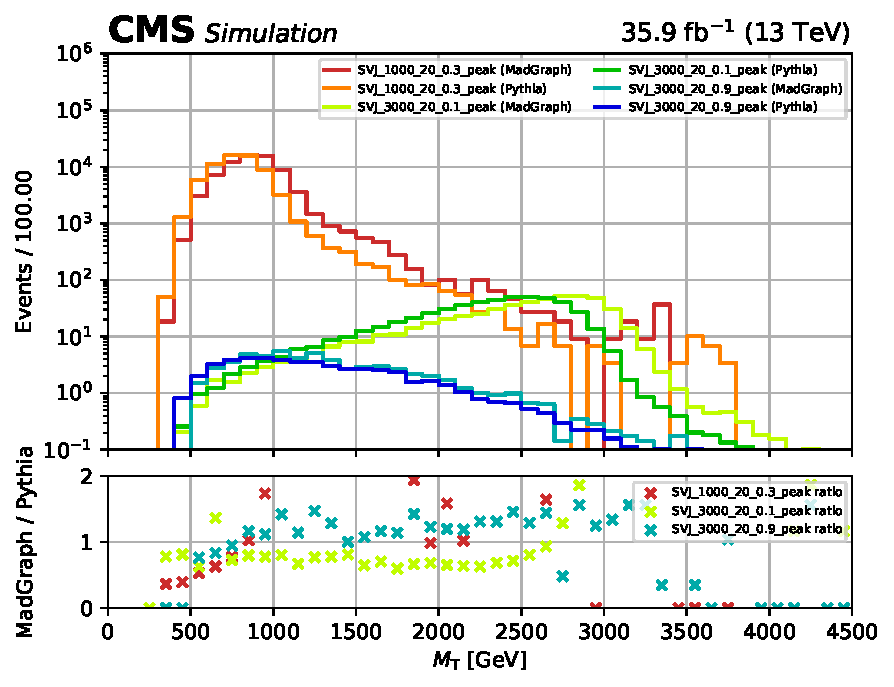
\includegraphics[width=\textwidth]{figures/madgraph_pythia_comparisons/with_ratios/part1/dijet_mt.pdf}
        \caption{Transverse mass of the dijet system}
    \end{subfigure}
    \hfill
    \begin{subfigure}[b]{0.45\textwidth}
        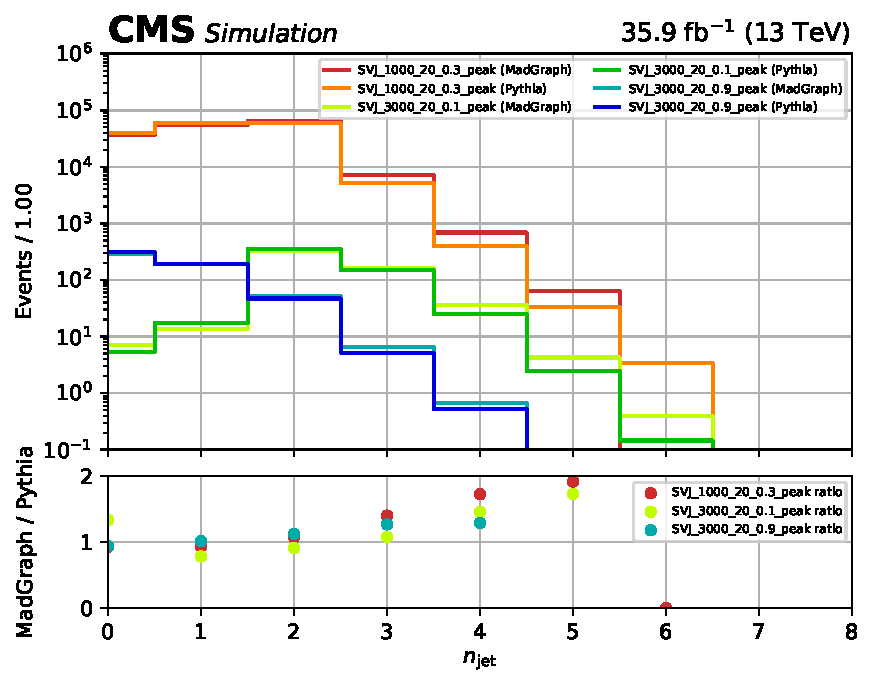
\includegraphics[width=\textwidth]{figures/madgraph_pythia_comparisons/with_ratios/part1/njet.pdf}
        \caption{\njet}
    \end{subfigure}

    \begin{subfigure}[b]{0.45\textwidth}
        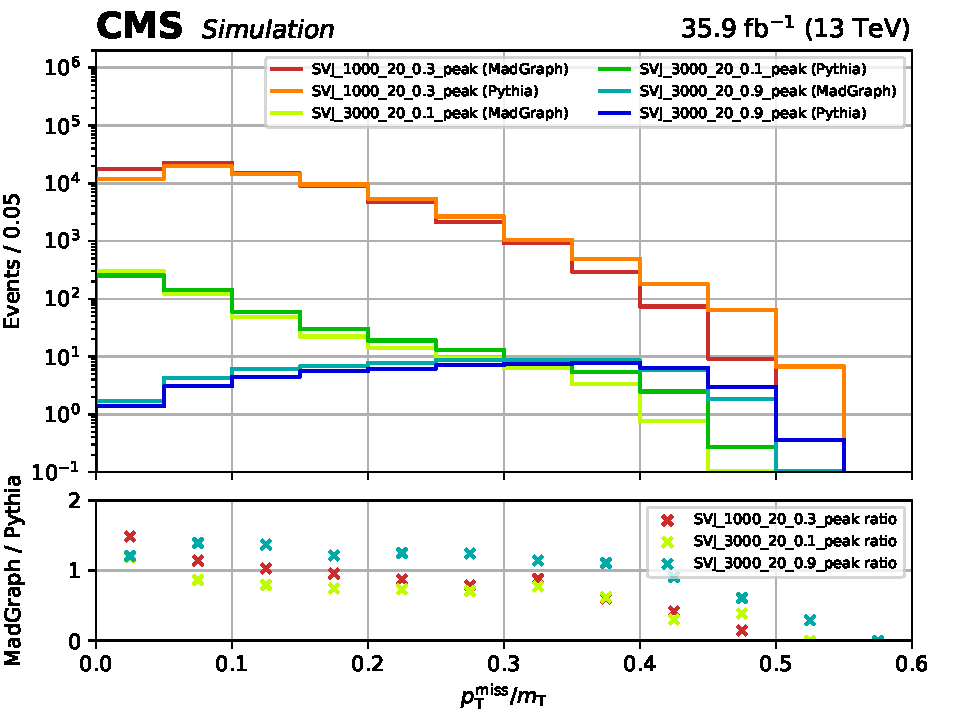
\includegraphics[width=\textwidth]{figures/madgraph_pythia_comparisons/with_ratios/part1/met_over_mt.pdf}
        \caption{$\MET/\mT$}
    \end{subfigure}
    \hfill
    \begin{subfigure}[b]{0.45\textwidth}
        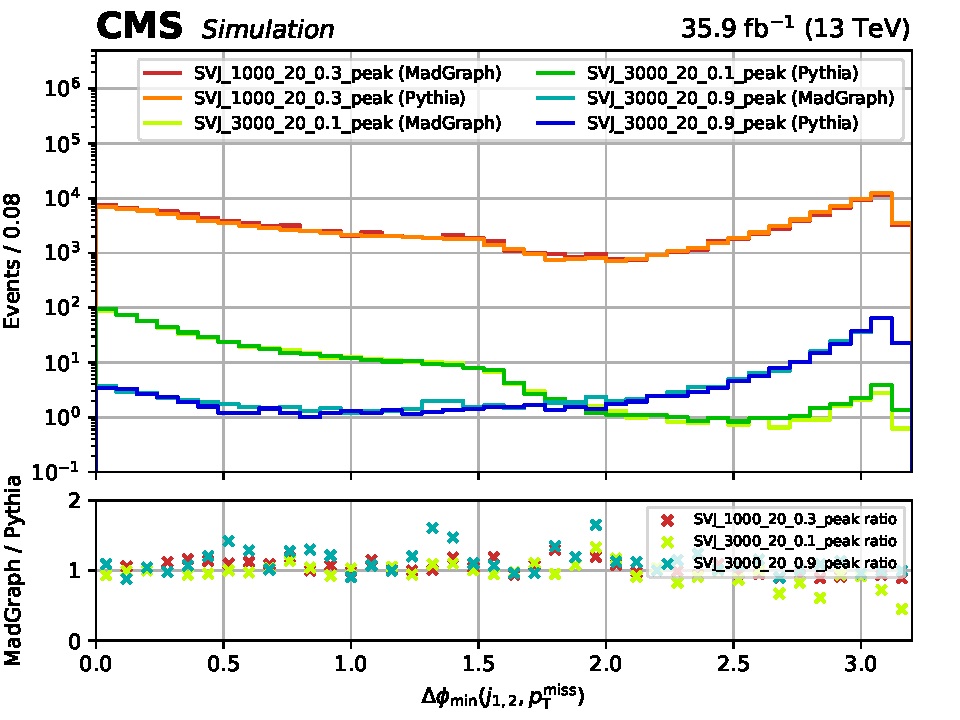
\includegraphics[width=\textwidth]{figures/madgraph_pythia_comparisons/with_ratios/part1/min_dphi.pdf}
        \caption{\mindphi between \MET and two leading \glspl{jet}}
    \end{subfigure}
    \caption[Distributions of several observables for the models SVJ\_1000\_20\_0.3\_peak, SVJ\_3000\_20\_0.1\_peak, and SVJ\_3000\_20\_0.9\_peak]{Distributions of several observables for the models SVJ\_1000\_20\_0.3\_peak, SVJ\_3000\_20\_0.1\_peak, and SVJ\_3000\_20\_0.9\_peak. Generation in \MGvATNLO is compared to \PYTHIAEIGHT, with the ratios between them for each model displayed in the respective subplot.}
    \label{fig:svj_mg_pythia_comparison_set1}
\end{figure}

\begin{figure}[htbp]
    \centering
    \begin{subfigure}[b]{0.45\textwidth}
        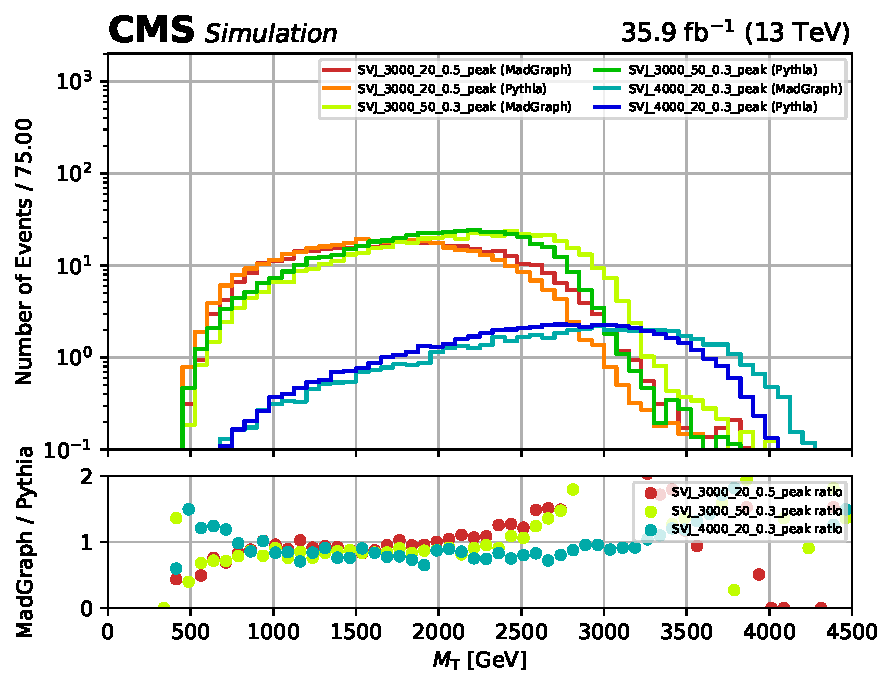
\includegraphics[width=\textwidth]{figures/madgraph_pythia_comparisons/with_ratios/part2/dijet_mt.pdf}
        \caption{Transverse mass of the dijet system}
    \end{subfigure}
    \hfill
    \begin{subfigure}[b]{0.45\textwidth}
        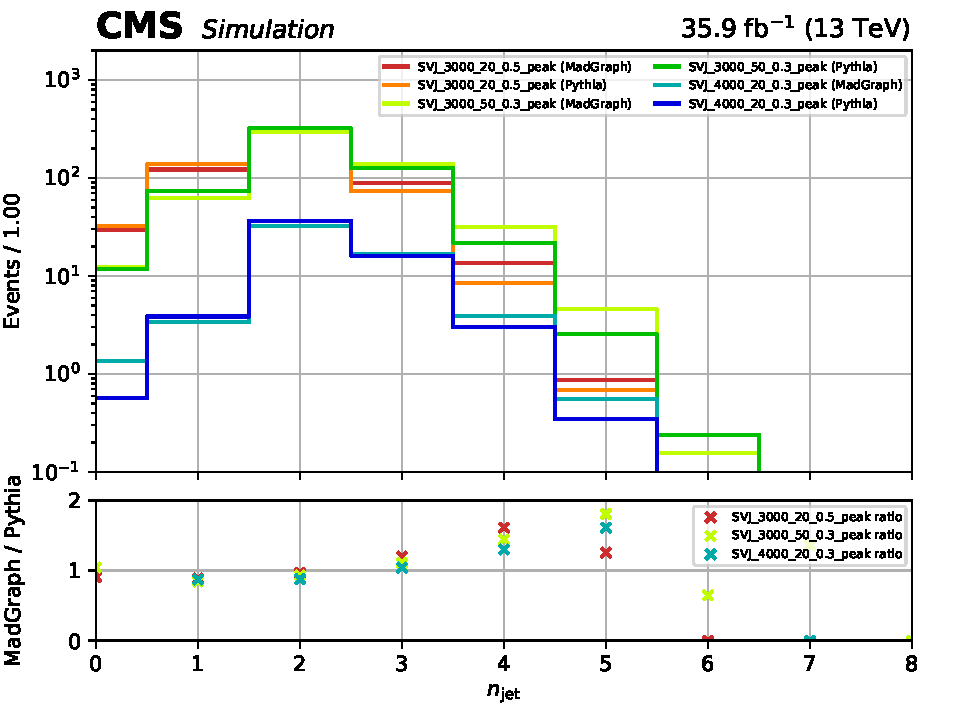
\includegraphics[width=\textwidth]{figures/madgraph_pythia_comparisons/with_ratios/part2/njet.pdf}
        \caption{\njet}
    \end{subfigure}

    \begin{subfigure}[b]{0.45\textwidth}
        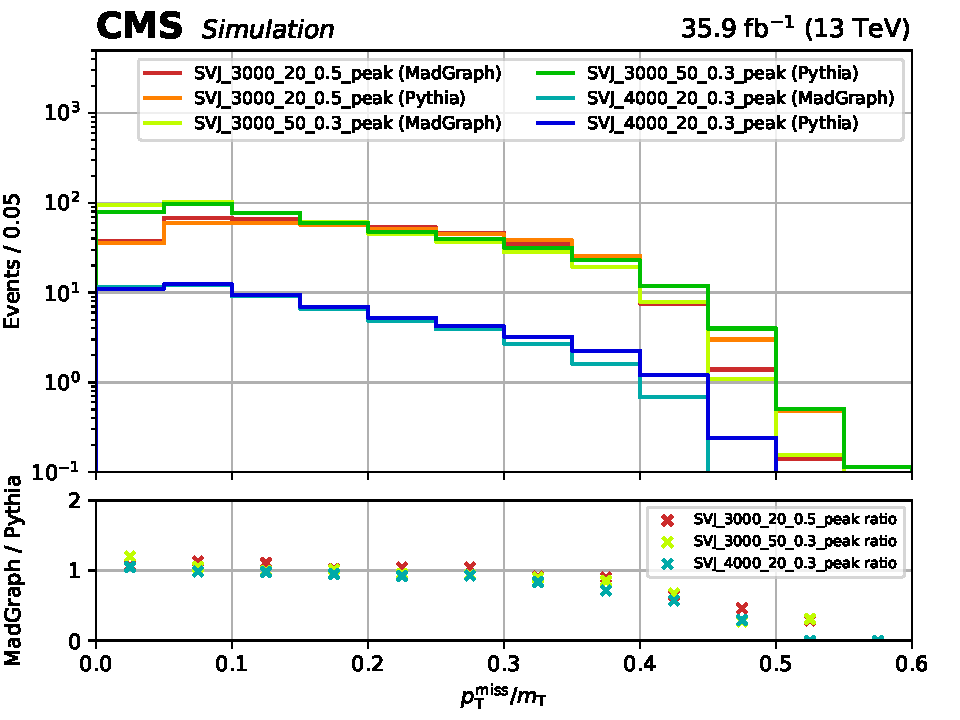
\includegraphics[width=\textwidth]{figures/madgraph_pythia_comparisons/with_ratios/part2/met_over_mt.pdf}
        \caption{$\MET/\mT$}
    \end{subfigure}
    \hfill
    \begin{subfigure}[b]{0.45\textwidth}
        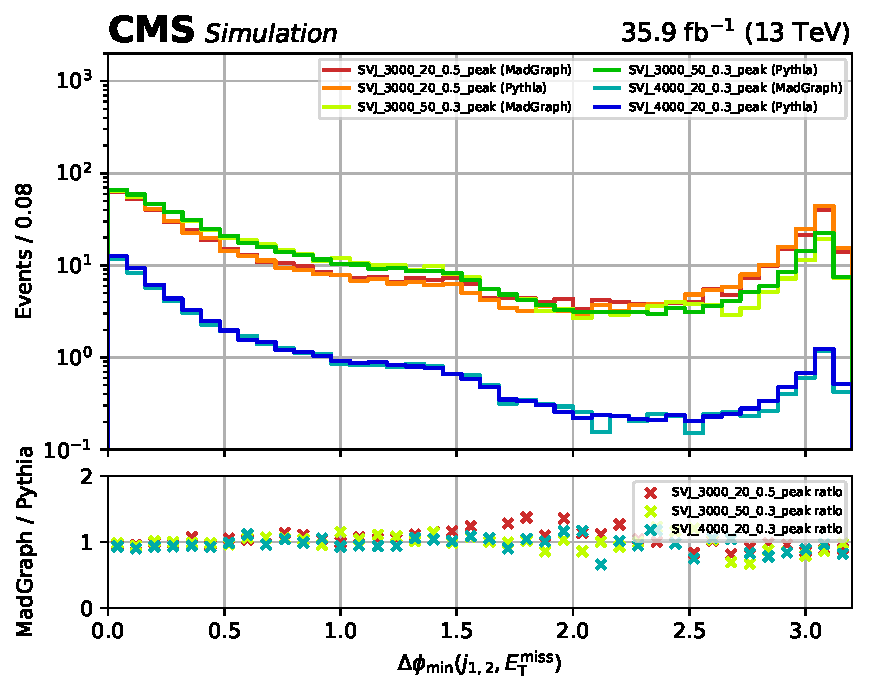
\includegraphics[width=\textwidth]{figures/madgraph_pythia_comparisons/with_ratios/part2/min_dphi.pdf}
        \caption{\mindphi between \MET and two leading \glspl{jet}}
    \end{subfigure}
    \caption[Distributions of several observables for the models SVJ\_3000\_20\_0.5\_peak, SVJ\_3000\_50\_0.3\_peak, and SVJ\_4000\_20\_0.3\_peak]{Distributions of several observables for the models SVJ\_3000\_20\_0.5\_peak, SVJ\_3000\_50\_0.3\_peak, and SVJ\_4000\_20\_0.3\_peak. Generation in \MGvATNLO is compared to \PYTHIAEIGHT, with the ratios between them for each model displayed in the respective subplot.}
    \label{fig:svj_mg_pythia_comparison_set2}
\end{figure}

% Show that the min_dphi shows stuff similar to WIMPs for high r_inv (maximum at pi). And at low r_inv, peaks close to 0 and pi, so MET is likely to be within a jet or recoiling from it

% For njet, typically see 2 jets as expected. Sometimes, an initial jet can be large enough to be clustered as two jets

% Generating 100,000 events. Obviously fewer end up in the plots from jet matching and filter efficiency
